\documentclass[12pt]{article}
\usepackage{longtable}
\usepackage{graphicx}
\usepackage[colorlinks=true]{hyperref}
\begin{document}
\author{\href{http://freecol.sourceforge.net/index.php?section=8}
  {The FreeCol Team}}
\title{FreeCol Documentation\\User Guide for Version v0.5.3}
\maketitle{}

\tableofcontents

\hypertarget{Introduction}{\section{Introduction}}

Welcome to FreeCol! If you're interested in development of this
program, please see the \href{http://freecol.sourceforge.net}{FreeCol
web site}. This is a draft version of the user's guide. You can find
the latest version at the
\href{http://freecol.sourceforge.net}{FreeCol homepage}.

%% \hypertarget{History}{\section{History}}
%% \label{history}
%% This section gives details about the history of this user guide.
%% \begin{itemize}
%% \item v0.2.0: add the �About� section and disband shortcut.
%% \item v0.1.2: corrections from Bryce Harrington and copyright notice.
%% \item v0.1.1: Main screen's, Colony panel's and Europe panel's images
%%   were added.
%% \item v0.1: Creation of the user guide! The guide contains the
%%   following sections: �Introduction�, �History�, �Installation� and
%%   �Interface�.
%% \end{itemize}

\hypertarget{About}{\section{About}}

\hypertarget{About FreeCol}{\subsection{About FreeCol}}

The FreeCol team aims to create an Open Source version of
Colonization (released under the
\href{http://www.gnu.org/licenses/gpl.html}{GPL}). At
first we'll try to make an exact clone of Colonization. The visuals
will be brought up to date with more recent standards but will remain
clean, simple and functional. Certain new 'features' will be
implemented but the gameplay and the rules will be exactly the same as
the original game. Examples of modern features are: an isometric map
and multiplayer support.

This clone will be developed incrementally and result in
\textbf{FreeCol 1.0.0 which will be an almost exact Colonization
clone}. Incremental development basically means that we'll add
features one at a time. This allows us to have a running program at
all times and also to release an unfinished but working game once in a
while.

Once FreeCol 1.0.0 is finished we'll start working towards FreeCol
2.0.0. \textbf{FreeCol 2 will go beyond the original Colonization} and
will have many new features, it will be an implementation of our (and
our users') image of what Colonization 2 would have been.

\hypertarget{The Original Colonization}{\subsection{The Original Colonization}}

The original Colonization was released in 1994 by Microprose.
\textbf{Colonization is heavily based on Civilization} which is
generally considered to be the best turn-based strategy game for the
PC in the history of mankind.

In Civilization the object of the game was to build a nation that
could stand the test of times and that could also do one of the
following: conquer the world or be the first to launch a
spaceship. In Colonization things are bit different...

A Colonization game starts in 1492 and \textbf{the object of the game
is to colonize America}. You begin the game with one vessel and two
colonists.

As in Civilization you need to build a powerful nation, but
fortunately in the early part of the game \textbf{you'll be able to
send ships back to Europe} in order to sell the goods you've produced
or to bring back some colonists. \textbf{Getting colonists into the
new world is a very important aspect of the game} as one game turn
takes one year and later on even one season and as a result colonies
don't grow as rapidly as they do in Civilization. You can pay
colonists to come to the new world or you can show off with the
religious freedom of your people in which case they will hop on your
vessels for no money at all.

Another important aspect is \textbf{trade: the source of all income}
(apart from Inca and Aztec gold). In a land filled with precious
resources it is important to \textbf{build your colonies at the right
location} and to place crafstmen where they belong. This is not only
to have an income but also to be able to \textbf{live off the land}
when you can no longer count on the support of Europe.

Through all this you'll have to decide whether or not you want to
\textbf{live next to the native americans} peacefully. They can teach
your colonists new skills that cannot be tought anywhere else and they
will offer you goods in case you choose to treat them as your
friends. On the other hand, their villages can be attacked and their
valuable goods can be taken from them and sold in Europe.

\textbf{Other European forces are also busy occupying their piece of
the new world}. Should their borders go too far then take over some
of their colonies by force because they wouldn't hesitate to do the
same thing to you.

The object of Colonization is to \textbf{declare your independence and
survive an attack of the King's forces}. Before declaring your
independence \textbf{you need to have the majority of the people
behind you}. This can be done by \textbf{promoting free speech} and by
providing a strong governmental system.

\hypertarget{Installation}{\section{Installation}}

To compile FreeCol you'll need Java and the Ant build system. FreeCol
is known to work with Sun's Java 1.4 and 5, but not with projects
based on GNU Classpath, as some font handling classes used by FreeCol
have not yet been implemented. Ant can be found at \href{Ant
homepage}{http://ant.apache.org/}.

When these are installed, go to the root directory of FreeCol and type
\verb$ant$ to build a JAR file containing the game. The game is
started using the command \verb$java -Xmx256M -jar FreeCol.jar$.  If
something goes wrong, send a bug report at the
\href{http://sourceforge.net/projects/freecol}{SourceForge page of
FreeCol}.

\hypertarget{Interface}{\section{Interface}}

This section will provide information about the keyboard shortcuts and
the different actions that can be used in the game.

\hypertarget{The main screen}{\subsection{The main screen}}

The figure \ref{main_screen_fig} represents the main screen.
\begin{figure}[htb]
  \begin{center}
    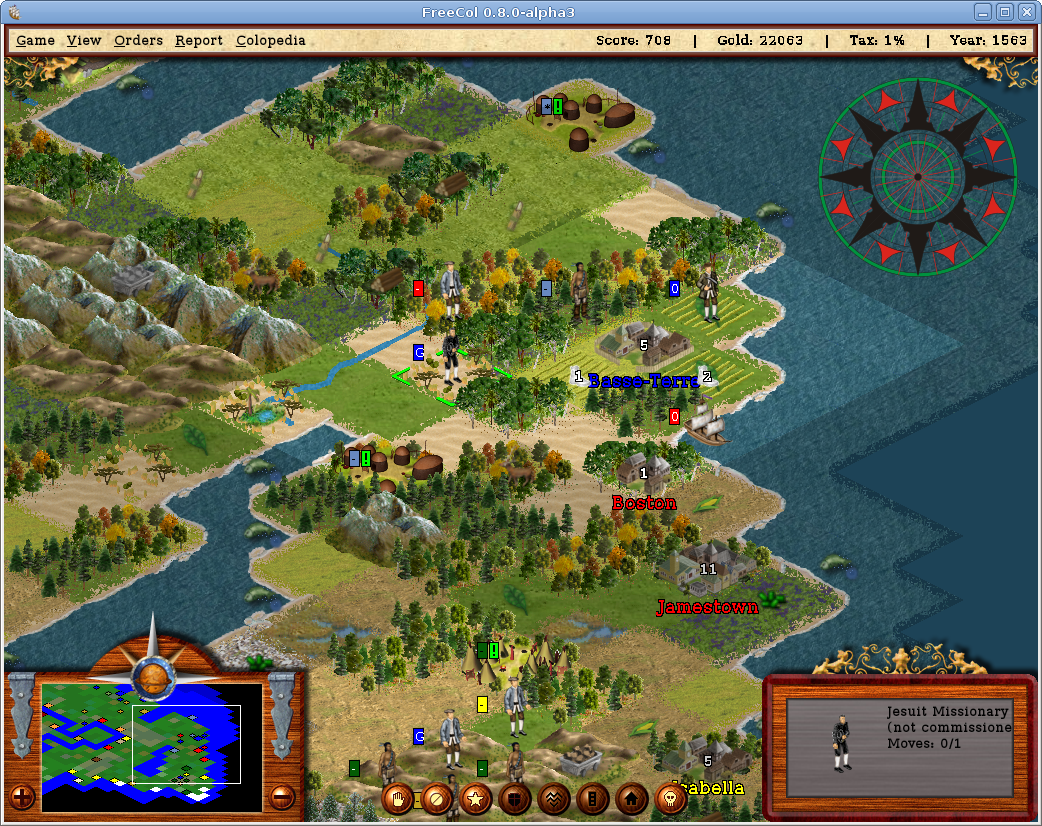
\includegraphics[scale=0.35]{images/main_screen.png}
    \caption{The main screen.\label{main_screen_fig}}
  \end{center}
\end{figure}

The units, colonies, and so forth can be seen on the main screen. You
can change the currently selected unit by clicking on any other
unit. You can move the currently selected unit using the numeric
keypad. If you select a unit with the left mouse button and drag the
mouse, the main screen will display the best path from the unit's
current position to the tile the mouse is hovering over. 

The tiles the path consists of will be marked with boots if the unit
is on foot, with horseshoes if the unit is mounted, with wheels if the
unit is a wagon train, or with sextants if the unit is a naval
unit. Full-colour symbols mark tiles that can be reached in the same
turn, whereas shaded symbols mark tiles that can be reached only in
subsequent turns. A number indicates how many turns later the unit
will arrive on this tile. 

  \begin{center}
    
\includegraphics{../data/images/ui/path-foot.png}
    
\includegraphics{../data/images/ui/path-horse.png}
    
\includegraphics{../data/images/ui/path-wagon.png}
    
\includegraphics{../data/images/ui/path-naval.png}
  \end{center}


Once you release the mouse button, the selected unit will begin to
follow this path. It will awake once it has arrived at its destination
or if it can no longer follow the path (if a unit belonging to a
different player is in the way, for instance).

If you right click on a tile containing neither units nor settlements,
a popup window will show you some information about the goods that can
be produced on this tile (unless the tile has not yet been explored,
in which case nothing will happen). If the tile contains units or
settlements, you will be presented with a menu from which you can
select the units or the settlement present, or the tile information.

The following shortcuts are also available:
\begin{itemize}
\item\verb$b$: build a colony.
\item\verb$c$: center on the currently selected unit.
\item\verb$d$: disband the active unit.
\item\verb$e$: show the Europe panel.
\item\verb$f$: fortify.
\item\verb$g$: goto some destination.
\item\verb$p$: plow the current tile.
\item\verb$r$: build a road on the current tile.
\item\verb$s$: sentry (not implemented).
\item\verb$w$: wait.
\item\verb$space$: skip for this turn.
\item\verb$enter$: end the turn.
\item\verb$plus$ or \verb$equals$: zoom in.
\item\verb$minus$ or \verb$underscore$: zoom out.
\item\verb$ctrl-d$: display tile names.
\item\verb$ctrl-g$: display grid.
\item\verb$ctrl-m$: show/hide the map controls.
\item\verb$ctrl-n$: new game.
\item\verb$ctrl-o$: open a game.
\item\verb$ctrl-q$: quit the game.
\item\verb$ctrl-r$: reconnect.
\item\verb$ctrl-s$: save a game.
\item\verb$ctrl-t$: show the chat panel.
\end{itemize}

\hypertarget{The Europe panel}{\subsection{The Europe panel}}

The figure \ref{europe_panel_fig} represents the Europe panel.
\begin{figure}[htb]
  \begin{center}
    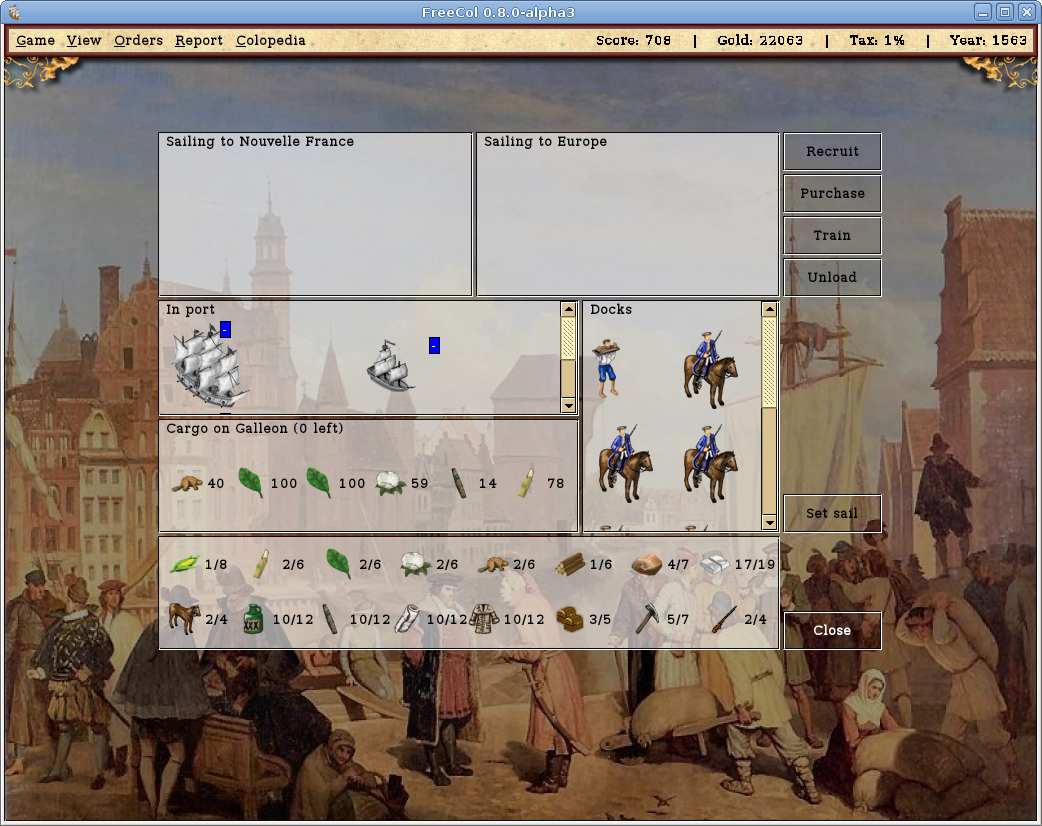
\includegraphics[scale=0.35]{images/europe_panel.png}
    \caption{The Europe Panel.\label{europe_panel_fig}}
  \end{center}
\end{figure}

In this panel, you can control the ships embarked for America or Europe,
and the ships currently stationed in Europe. You can also buy goods,
recruit, purchase and train units. Units recruited, purchased or trained
are in the �Docks� area in the Europe panel.

If a ship has set sail for Europe or America, you can change its
direction by dragging it from the �Going to America� box to the �Going
to Europe� box (or vice versa).

Ships that are docked at the European port can also do the following:
\begin{itemize}
\item Embark/Disembark units: drag and drop between the �Docks�
  and �Cargo� sections of the Europe panel.
\item Sell/Buy goods: drag and drop between the �Cargo� panel and the
  �Market� panel. If you want to sell only a part of your cargo, or
  want to buy less than 100 units of goods, press the shift key while
  dragging. This will allow you to specify how many units you wish to
  transfer. If any of the goods are displayed in grey, this means they
  are being boycotted by the Crown because you refused a tax
  raise. You must pay your tax arrears before you can trade these
  goods. You can do this by dragging the goods as usual, in which case
  you will be given the chance to pay your tax arrears (provided you
  have enough money).
\item Arm/Mount/Equip with tools/Dress as missionaries a unit: 
  right click on the unit.
\item Move your ship to the �Going to America� section of the Europe
  panel.
\end{itemize}

\hypertarget{The Colony panel}{\subsection{The Colony panel}}

The figure \ref{colony_panel_fig} represents the Colony panel.
\begin{figure}[htb]
  \begin{center}
    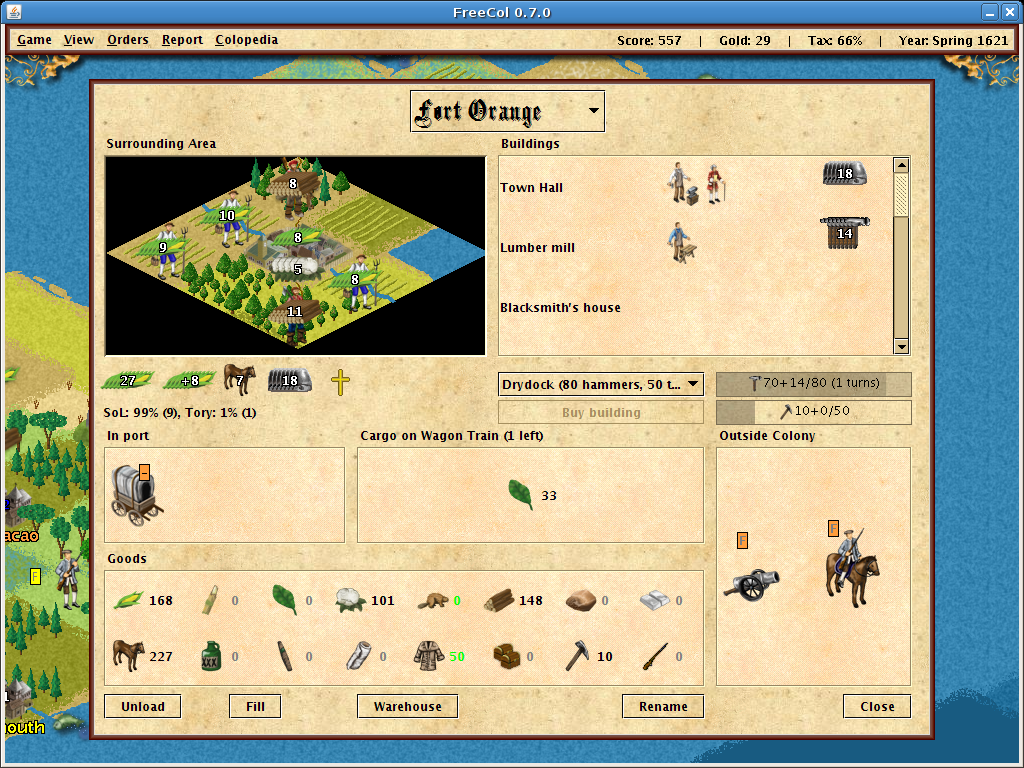
\includegraphics[scale=0.35]{images/colony_panel.png}
    \caption{The Colony Panel.\label{colony_panel_fig}}
  \end{center}
\end{figure}

To view a colony's panel, left click on it from the main
screen. From this panel, colonist's cultivation, production, and other
tasks can be assigned:

\begin{itemize}
\item Cultivation: Drop the unit onto the appropriate plot of land in
  the colony. You can change what a colonist cultivate by right
  clicking on it. Note that your colonists can not go fishing on ocean
  tiles before they have built a dock.
\item Production: Drop the unit onto the relevant �Buildings�.
\item Depart colony: Drop the unit onto the colony's gate.
\item Embark on a ship: If there is a ship in port, you can embark
  your colonist on it by dropping it onto the �Cargo� section of the
  colony panel.
\item Build a building: Drop the unit onto the carpenter's house and
  select the building you want from the building menu.
\end{itemize}

You can also load cargo into a ship's hold by dropping the goods onto
the ship or the specific hold within the ship. Use the shift key while
dropping it if you want to load only a portion of the goods.


\hypertarget{The New World}{\section{The New World}}

At the beginning of the game, you will start with a naval vessel and
two colonists. Your first task will be to discover the New World,
which should lie due West, although sailing North or South may prove
quicker. As soon as you have discovered land, you can establish your
colonies and produce goods to send home to Europe.

\hypertarget{Terrain Types}{\subsection{Terrain Types}}

There are many different types of terrain in the New World, each with
its own peculiar advantages. At the beginning of the game you will
probably arrive at a \hypertarget{High Seas}{\textbf{High Seas}} tile
(or at the edge of the map). High Seas tiles (and the map edge) allow
you to sail between Europe and the New World. As you approach land,
the High Seas will be replaced by \hypertarget{Ocean}{\textbf{Ocean}}
tiles, which produce \hyperlink{Fish}{Fish}.

In the New World, you will also discover
\hypertarget{Plains}{\textbf{Plains}}, which produce a great deal of
Grain, a lesser amount of Cotton, and some Ore;
\hypertarget{Grassland}{\textbf{Grassland}}, on which Grain and
Tobacco can be cultivated; \hypertarget{Prairie}{\textbf{Prairies}},
which are suitable for growing Grain and Cotton;
\hypertarget{Savannah}{\textbf{Savannah}}, which produces Grain and
Sugar; \hypertarget{Marsh}{\textbf{Marsh}}, where Grain can be
cultivated and some Ore can be mined;
\hypertarget{Swamp}{\textbf{Swamp}}, which yields some Grain, and
small amounts of Sugar, Tobacco and Ore;
\hypertarget{Desert}{\textbf{Deserts}}, which produce some Food,
Cotton and Ore; as well as \hypertarget{Tundra}{\textbf{Tundra}},
where Grain can be grown, and some Ore can be mined.

Large parts of the New World are covered in forests, all of which
yield varying amounts of Grain, Lumber and Furs. The
\hypertarget{Boreal Forest}{\textbf{Boreal Forest}} also produces Ore,
the \hypertarget{Mixed Forest}{\textbf{Mixed Forest}} Cotton, the
\hypertarget{Conifer Forest}{\textbf{Conifer Forest}} Tobacco, the
\hypertarget{Tropical Forest}{\textbf{Tropical Forest}} Sugar, the
\hypertarget{Rain Forest}{\textbf{Rain Forest}} produces small amounts
of Ore, Sugar and Tobacco, the \hypertarget{Wetland
Forest}{\textbf{Wetland Forest}} and the \hypertarget{Scrub
Forest}{\textbf{Scrub Forest}} yield some Ore, and the
\hypertarget{Broadleaf Forest}{\textbf{Broadleaf Forest}} Cotton.

The \hypertarget{Hills}{\textbf{Hills}} produce a small amount of
Grain, and can be mined for Ore and a lesser amount of Silver. The
\hypertarget{Mountains}{\textbf{Mountains}} are unsuitable for
agriculture, but yield some Ore and
Silver. \hypertarget{Arctic}{Arctic} tiles are the least useful type
of terrain, as they produce nothing at all. Terrain types that produce
no Grain, such as the Mountains and Artic types, can not support
colonies.

The New World is also irrigated by minor and major rivers. The
prouction of most types of \hyperlink{Goods}{Goods} is increased by
the presence of rivers and roads, which your
\hyperlink{Pioneer}{Pioneers} can build. All terrain types which
produce Grain (except the Hills) can also be cleared or plowed by your
Pioneers. In the case of open land, plowing increases the production
of Grain and most other types of goods. In the case of forests,
clearing removes the forest and transforms the tile into open land:
Boreal Forest is transformed into Tundra, Mixed Forest into Plains,
Conifer Forest into Grassland, Tropical Forest into Savannah, Wetland
Forest into Marsh, Rain Forest into Swamp, Scrub Forest into Desert,
and Broadleaf Forest into Prairie.


\hypertarget{Colonies}{\section{Colonies}}

\hypertarget{Picking a suitable site}{\subsection{Picking a suitable site}}

Your colonies are your most important assets in the new world.
Therefore, it is very important to build them in the right
place. There are several aspects to consider:

\hypertarget{The colony tile}{\subsubsection{The colony tile}}

Some terrain types are more suitable for establishing a colony than
others. Colonies can not be built on arctic tiles, nor on
mountains. Hills and deserts are less suitable than other tiles
because they produce less food, which is very important in the long
run. Tiles with forest generally produce less food than tiles without,
but pioneers are able to cut down the forest and plow the tile, which
will increase food production. The presence of a river will also
increase food production.

\hypertarget{The adjacent tiles}{\subsubsection{The adjacent tiles}}

In the early stages of the game, you will need to generate cash by
selling products from the New World in your Home Port. Thus, many of
your early colonies should probably be situated next to bonus tiles,
which greatly increase production. Rivers also increase production,
though not as much as a bonus resource. On the other hand, they
increase the production of many different kinds of goods, unlike a
bonus resource.

In order to improve your colony, you will have to construct various
buildings. This will require large amounts of lumber. For this reason,
you should make sure that at least one tile adjacent to your colony
site can produce sufficient amounts of lumber. You will also need
tools to construct advanced buildings. Therefore, it is an advantage
if the colony can also produce ore, which can be refined to produce
tools. However, ore is not as important as lumber.

Some of the tiles may be owned by other European powers, or claimed by
Indians. Building a colony too close to other settlements is not a
good idea, unless you plan to conquer or destroy these settlements.
But remember that colonies with a \hyperlink{Stockade}{Stockade} can
not be abandoned.  Keeping your own colonies close together is a good
strategy, however, as long as you avoid sharing tiles between several
colonies as far as possible.

\hypertarget{No Reforestation}{\subsubsection{No Reforestation}}

You can order your pioneers to cut down forests by plowing a tile.
This will increase the food produced on these tiles, and the lumber
will be delivered to your colonies. However, you can not plant new
forests later. Once cleared, a tile will never produce lumber again.

\hypertarget{Colony Buildings}{\subsection{Colony Buildings}}

A newly established colony already includes several buildings, namely
a town hall, a carpenter's house, a blacksmith's house, a
tobacconist's house, a weaver's house, a distiller's house, a fur
trader's house, and a warehouse. You can improve your colonies by
upgrading all of these buildings except the town hall, and by
constructing various new buildings. However, many buildings can only
be constructed in colonies of a certain size, or after certain
\hyperlink{Founding Fathers}{Founding Fathers} have joined the
\hyperlink{Continental Congress}{Continental Congress}.

The craftsmen's houses can be upgraded to workshops, which produce
more manufactured goods. After \hyperlink{Adam Smith}{Adam Smith} has
joined the \hyperlink{Continental Congress}{Continental Congress},
workshops can be upgraded to factories, which produce one and a half
units of manufactured goods from each unit of raw material. While the
town hall itself can not be upgraded, the production of
\hyperlink{Liberty Bells}{Liberty Bells} can be boosted by
constructing a printing press and then a newspaper.

All in all, there are sixteen different buildings, eight of which are
part of every newly established colony:

\begin{itemize}
\item The \hypertarget{Town Hall}{\textbf{Town Hall}}, which can not
  be upgraded, provides workplaces for up to three colonists producing
  \textbf{Liberty Bells}. Its effect can be increased by building a
  \hyperlink{Printing Press}{Printing Press} and a
  \hyperlink{Newspaper}{Newspaper}.

\item The \hypertarget{Carpenter's House}{\textbf{Carpenter's House}},
  which can be upgraded to a \textbf{Lumber Mill} once the colony's
  population reaches 3, is used to convert \hyperlink{Lumber}{Lumber}
  to \hyperlink{Hammers}{Hammers}. Hammers are required to construct
  or upgrade all kinds of buildings.

\item The \hypertarget{Blacksmith's House}{\textbf{Blacksmith's
  House}}, which can be upgraded to a \hypertarget{Blacksmith's
  Workshop}{\textbf{Blacksmith's Workshop}}, is used to convert
  \hyperlink{Ore}{Ore} to \hyperlink{Tools}{Tools}. Tools are required
  to construct certain kinds of buildings and to upgrade all kinds of
  buildings. Tools are also used by \hyperlink{Pioneers}{Pioneers} and
  to produce \hyperlink{Muskets}{Muskets}. Once the population of the
  colony has reached 8, the Blacksmith's Workshop can be replaced by
  \hypertarget{Iron Works}{\textbf{Iron Works}}, provided that
  \hyperlink{Adam Smith}{Adam Smith} has joined the
  \hyperlink{Continental Congress}{Continental Congress}.

\item The \hypertarget{Tobacconist's House}{\textbf{Tobacconist's
  House}}, which can be upgraded to a \hypertarget{Tobacconist's
  Shop}{\textbf{Tobacconist's Shop}}, is used to produce
  \hyperlink{Cigars}{Cigars} from \hyperlink{Tobacco}{Tobacco}.  Once
  the colony's population has reached 8, it can be further upgraded to
  a \hypertarget{Cigar Factory}{\textbf{Cigar Factory}}, provided that
  \hyperlink{Adam Smith}{Adam Smith} has joined the
  \hyperlink{Continental Congress}{Continental Congress}.

\item The \hypertarget{Weaver's House}{\textbf{Weaver's House}},
  which can be upgraded to a \hypertarget{Weaver's
  Shop}{\textbf{Weaver's Shop}}, is used to turn
  \hyperlink{Cotton}{Cotton} into \hyperlink{Cloth}{Cloth}. It can be
  upgraded to a \hypertarget{Textile Mill}{\textbf{Textile Mill}} as
  soon as the population of the colony is at least 8 and
  \hyperlink{Adam Smith}{Adam Smith} has joined the
  \hyperlink{Continental Congress}{Continental Congress}.

\item The \hypertarget{Distiller's House}{\textbf{Distiller's
  House}}, which can be upgraded to a \hypertarget{Rum
  Distillery}{\textbf{Rum Distillery}}, is used to produce
  \hyperlink{Rum}{Rum} from \hyperlink{Sugar}{Sugar}. Once
  \hyperlink{Adam Smith}{Adam Smith} has joined the
  \hyperlink{Continental Congress}{Continental Congress} and the
  colony's population is at least 8, the rum distillery can be
  replaced by a \hypertarget{Rum Factory}{\textbf{Rum Factory}}.

\item The \hypertarget{Fur Trader's House}{\textbf{Fur Trader's
  House}}, which can be upgraded to a \hypertarget{Fur Trader's
  Post}{\textbf{Fur Trader's Post}}, is used to produce
  \hyperlink{Coats}{Coats} from \hyperlink{Fur}{Fur}. Once the
  colony's population has reached 6, it can be further upgraded to a
  \hypertarget{Fur Factory}{\textbf{Fur Factory}}, provided that
  \hyperlink{Adam Smith}{Adam Smith} has joined the
  \hyperlink{Continental Congress}{Continental Congress}.

\item The \hypertarget{Warehouse}{\textbf{Warehouse}} stores all kinds
  of goods. Its initial capacity is 100 units of each kind of goods,
  but it can be upgraded to 200 and finally 300 units.
\end{itemize}

The following eight buildings are not part of your basic colony and
have to be constructed later:

\begin{itemize}
\item A colony with a population of at least 4 may build a 
  \hypertarget{Schoolhouse}{\textbf{Schoolhouse}}, which enables some
  master craftsman to teach an unskilled colonist their trade. As soon
  as the population reaches 8, it can be upgraded to a
  \hypertarget{College}{\textbf{College}}, in which additional trades
  can be taught by two colonists. Once the population reaches 10, the
  college can be replaced by a
  \hypertarget{University}{\textbf{University}}, at which all trades
  can be taught by three colonists. See \hyperlink{Skills and
  Education}{Skills and Education} for details.

\item The \hypertarget{Armory}{\textbf{Armory}} is used to produce
  \hyperlink{Muskets}{Muskets} from \hyperlink{Tools}{Tools}. As soon
  as the population reaches 8, the armory can be upgraded to a
  \hypertarget{Magazine}{\textbf{Magazine}} and then to an
  \hypertarget{Arsenal}{\textbf{Arsenal}}, provided that
  \hyperlink{Adam Smith}{Adam Smith} has joined the
  \hyperlink{Continental Congress}{Continental Congress}.

\item A colony with a population of 3 or more may build a
  \hypertarget{Church}{\textbf{Church}}, which can be upgraded to a
  \hypertarget{Cathedral}{\textbf{Cathedral}} as soon as the
  population reaches 8. The religious freedom of the New World
  (symbolized by \hyperlink{Crosses}{Crosses}) causes increased
  emigration from Europe.

\item The \hypertarget{Stockade}{\textbf{Stockade}}, which can be
  constructed as soon as the colony's population reaches 3, protects
  the colonists from attacks. Note that a colony with a stockade can
  not be abandoned, it can only be burned to the ground by
  natives. The stockade can be upgraded to a
  \hypertarget{Fort}{\textbf{Fort}}, which provides better protection
  and bombards \hyperlink{Privateers}{Privateers} and enemy naval
  units on adjacent ocean tiles. The fort can be replaced by a
  \hypertarget{Fortress}{\textbf{Fortress}} as soon as the population
  reaches 8.

\item The \hypertarget{Stables}{\textbf{Stables}} increase the
  production of \hyperlink{Horses}{Horses}.

\item The \hypertarget{Dock}{\textbf{Dock}} allows colonists to 
  produce \hyperlink{Fish}{Fish} on ocean tiles adjacent to the
  colony. As soon as the population is at least 4, it can be upgraded
  to a \hypertarget{Drydock}{\textbf{Drydock}}, which allows the
  colony to repair damaged ships. When the colony's population reaches
  8, it can be further upgraded to a
  \hypertarget{Shipyard}{\textbf{Shipyard}}, which enables the colony
  to build new ships.

\item The \hypertarget{Printing Press}{\textbf{Printing Press}}, 
  which can be upgraded to a
  \hypertarget{Newspaper}{\textbf{Newspaper}} as soon as the
  population reaches 4, increases the colony's production of
  \hyperlink{Liberty Bells}{Liberty Bells}.

\item The \hypertarget{Custom House}{\textbf{Custom House}}, which can
  be built as soon as \hyperlink{Peter Stuyvesant}{Peter Stuyvesant}
  has joined the \hyperlink{Continental Congress}{Continental
  Congress}, allows the colony to export goods to Europe directly
  without the help of ships. Optionally, it may also ignore
  \hyperlink{Boycotts}{Boycotts}.

\end{itemize}



\hypertarget{Units}{\section{Units}}

Several dozen different units are available in FreeCol, but not all
units are available to all players. Some units are available only to
\textbf{Indian Players}, some units are only available to
\textbf{European Players}, and other units are available only to the
\textbf{Royal Expeditionary Force}.

The most basic unit of the European Players (including you) is the
\hypertarget{Free Colonist}{\textbf{Free Colonist}}. The Free
Colonist is quite good at any task, but has no special skills. At the
beginning of the game, many of the colonists will not be volunteers,
but \hypertarget{Indentured Servant}{\textbf{Indentured Servants}}, or
\hypertarget{Petty Criminal}{\textbf{Petty Criminals}}, who are
deported to the New World. Indentured Servants are pretty bad at all
jobs within the colony, but just like Free Colonists, they can be sent
to native villages to learn a skill from the natives. Petty Criminals
are very bad at all jobs within the colony and can not learn anything
from the natives. However, both Indentured Servants and Petty
Criminals can become Free Colonists through \hyperlink{Skills and
Education}{Education}.

Many early colonies failed due to a lack of food. In order to avoid a
similar fate, you must ensure adequate food production from the very
beginning. All your colonists can produce some amount of food,
especially on the more fertile terrain types, but \hypertarget{Expert
Farmer}{\textbf{Expert Farmer}} and the \hypertarget{Expert
Fisherman}{\textbf{Expert Fisherman}} will greatly increase your food
production. But note that the Expert Fisherman requires a
\hyperlink{Dock}{Dock} to moor his boat to, and that this requires at
least one ocean tile adjacent to your colony.

Three types of units are not available in Europe because they posses
skills that can only be learned from the native population. These are
the \hypertarget{Master Sugar Planter}{\textbf{Master Sugar Planter}},
the \hypertarget{Master Cotton Planter}{\textbf{Master Cotton
Planter}}, the \hypertarget{Master Tobacco Planter}{\textbf{Master
Tobacco Planter}}, and the \hypertarget{Expert Fur
Trapper}{\textbf{Expert Fur Trapper}}. These units are able to greatly
increase your production of \hyperlink{Sugar}{Sugar},
\hyperlink{Cotton}{Cotton}, \hyperlink{Tobacco}{Tobacco}, and
\hyperlink{Furs}{Furs}, respectively.

In the beginning of the game, you will most likely export a great deal
of these goods to Europe, but beware, prices will drop! However, all
the raw materials of the New World can be used to produce luxury goods
that will sell for higher prices in Europe. \hyperlink{Sugar}{Sugar}
can be used to distill \hyperlink{Rum}{Rum},
\hyperlink{Cotton}{Cotton} can be used to produce
\hyperlink{Cloth}{Cloth}, \hyperlink{Cigars}{Cigars} are made from
\hyperlink{Tobacco}{Tobacco}, and \hyperlink{Coats}{Coats} are made
from \hyperlink{Furs}{Furs}. All your colonists can do this, but the
\hypertarget{Master Distiller}{\textbf{Master Distiller}}, the
\hypertarget{Master Weaver}{\textbf{Master Weaver}}, the
\hypertarget{Master Tobacconist}{\textbf{Master Tobacconist}}, and the
\hypertarget{Master Fur Trader}{\textbf{Master Fur Trader}} are the
experts who will really rev up your production.

The New World also has two mineral resources, \hyperlink{Ore}{Ore} and
\hyperlink{Silver}{Silver}, to offer. Again, all your colonists are
able to mine these resources to a certain extent, but you will need
the \hypertarget{Expert Ore Miner}{\textbf{Expert Ore Miner}} and the
\hypertarget{Expert SilverMiner}{\textbf{Expert SilverMiner}} to make
the most of them.

\hyperlink{Lumber}{Lumber} can be produced in all forested tiles, and
can also be exported to Europe, although prices are low. However, you
will need vast amounts of lumber in order to upgrade your colonies,
and no colonist is more skilled at cutting down forests than the
\hypertarget{Expert LumberJack}{\textbf{Expert Lumberjack}}. Nor is
any colonist more skilled at turning the lumber into buildings than
the \hypertarget{Master Carpenter}{\textbf{Master Carpenter}}.

The more advanced buildings you can construct in the your colonies
require not only lumber but also \hyperlink{Tools}{Tools}, which are
produced from \hyperlink{Ore}{Ore}. This is the job the
\hypertarget{Master Blacksmith}{\textbf{Master Blacksmith}} excels in.
Tools are also used by your \hypertarget{Pioneer}{\textbf{Pioneers}}
to clear forests and plow fields, but none of your other colonists can
match the outdoors skills of your \hypertarget{Hardy
Pioneer}{\textbf{Hardy Pioneers}}. And finally, Tools are required for
the production of \hyperlink{Muskets}{Muskets}, a demanding task best
left to the \hypertarget{Master Gunsmith}{\textbf{Master Gunsmith}}.

All your units are able to explore the New World, but the colonist
most suited to this dangerous endeavour is the
\hypertarget{Scout}{\textbf{Scout}}, a mounted colonist. A Scout may
become a \hypertarget{Seasoned Scout}{\textbf{Seasoned Scout}} through
\hyperlink{Skills and Education}{experience}, either by visiting
native settlements, or by investigating \hyperlink{Lost City
Rumours}{Lost City Rumours}. The Seasoned Scout is much more skillful
at these jobs, but beware, they are dangerous!

Another colonist able to visit native settlements is the
\hypertarget{Missionary}{\textbf{Missionary}}. Any colonist can be
converted to a Missionary by blessing him in a colony with a
\hyperlink{Church}{Church}, or in the \hyperlink{Home Port}{Home
Port}, which is sure to have several churches and maybe even a
\hyperlink{Cathedral}{Cathedral}. Missionaries are able to establish a
\hyperlink{Mission}{Mission} in the native settlement, and to convert
the natives. \hypertarget{Jesuit Missionary}{\textbf{Jesuit
Missionaries}}, however, are much more accomplished at the job.

The converted natives may join your colonies as \hypertarget{Indian
Convert}{\textbf{Indian Converts}}. They are unskilled at all jobs
within the colony, but more skilled than your Free Colonists at all
outdoor jobs. Indian Converts can not be upgraded through
\hyperlink{Skills and Education}{Education}, but they become Free
Colonists as soon as \hyperlink{Bartolme de las Casas}{Bartolme de las
Casas} joins the \hyperlink{Continental Congress}{Continental
Congress}.

Many colonists come to the New World in search of religious
freedom. Thus, they desire a \hyperlink{Church}{Church} in which to
preach and pray. This religious freedom, which attracts more European
colonists, is represented by \hyperlink{Crosses}{Crosses}. Naturally,
some colonists are more eloquent and inspired than others, and the
most famous of these are known as \hypertarget{Firebrand
Preacher}{\textbf{Firebrand Preachers}}.

While the preachers are concerned with the spiritual welfare of the
colonists, the colonists concerned with the secular welfare of their
fellow citizens meet in the \hyperlink{Town Hall}{Town Hall}, which
generates \hyperlink{Liberty Bells}{Liberty Bells}. The most dignified
and influential of these citizens are considered \hypertarget{Elder
Statesman}{\textbf{Elder Statesmen}}.

Any colonist can be equipped with \hyperlink{Muskets}{Muskets}, which
makes him a \hypertarget{Soldier}{\textbf{Soldier}}, or a
\hypertarget{Dragoon}{\textbf{Dragoon}} if he is mounted. However,
combat-hardened \hypertarget{Veteran Soldier}{\textbf{Veteran
Soldiers}} and \hypertarget{Veteran Dragoon}{\textbf{Veteran
Dragoons}} are much more effective. A dragoon that is beaten in battle
is downgraded to a soldier. A beaten soldier becomes an unarmed
colonist. 

On the other hand, any soldier or dragoon that wins a battle may be
upgraded. A Petty Criminal will be upgraded to an Indentured Servant,
an Indentured Servant will be upgraded to a Free Colonist, and a Free
Colonist to a veteran unit. Veteran units may be further upgraded to
\hypertarget{Colonial Regular}{\textbf{Colonial Regulars}} or
\hypertarget{Colonial Cavalry}{\textbf{Colonial Cavalry}}, but only
after the \hyperlink{Declaration of Independence}{Declaration of
Independence}.

\hypertarget{Artillery}{\textbf{Artillery}} is most effective at
attacking and defending colonies and fortified units, but is also very
vulnerable in the open. Artillery may become damaged, which decreases
its efficiency. \hypertarget{Damaged Artillery}{\textbf{Damaged
Artillery}} is still quite powerful, but it can not be repaired, and
further damage will destroy it.

The \hypertarget{Wagon Train}{\textbf{Wagon Train}}, which has to be
built in one of your colonies, can be used to transport up to 200
units of goods over land and to trade with native settlements, and
foreign colonies if \hyperlink{Jan de Witt}{Jan de Witt} has joined
the \hyperlink{Continental Congress}{Continental Congress}.

The \hypertarget{Treasure Train}{\textbf{Treasure Train}} is similar
to the Wagon Train, but is used only to transport treasures. You can
find these treasures in \hyperlink{Lost City Rumours}{Lost Cities}, or
in the ruins of native settlements you have destroyed. If you move
your Treasure Trains into a colony with access to the sea, your
\hyperlink{Monarch}{Monarch} will offer to ship it to Europe for a
``reasonable fee'', unless \hyperlink{Hernan Cortes}{Hernan Cortes}
has joined the \hyperlink{Continental Congress}{Continental Congress},
in which case it will be shipped free of charge. If you have a
\hyperlink{Galleon}{Galleon}, however, you can take the Treasure Train
to Europe yourself.

The \hypertarget{Caravel}{\textbf{Caravel}}, the
\hypertarget{Merchantman}{\textbf{Merchantman}} and the
\hypertarget{Galleon}{\textbf{Galleon}} are unarmed naval units, with
two, four or six cargo holds, respectively. A cargo hold may contain
up to 100 units of goods, or any land unit except the Treasure Train,
which takes up six cargo holds all by itself, and the Wagon Train,
which can not be transported by sea at all.

The \hypertarget{Privateer}{\textbf{Privateer}} and the
\hypertarget{Frigate}{\textbf{Frigate}} are armed naval vessel with
two or four cargo holds, respectively. The Privateer is unique in that
it does not fly the flag of your country and can attack the vessels of
other countries with impunity. It becomes even more deadly when
\hyperlink{Francis Drake}{Francis Drake} joins the
\hyperlink{Continental Congress}{Continental Congress}.

The \hypertarget{Man of War}{\textbf{Man of War}} is the most powerful
naval vessel, and has six cargo holds. At the beginning of the game,
only the \hyperlink{Monarch}{Monarch} has these powerful ships, but
after the \hyperlink{Declaration of Independence}{Declaration of
Independence} you can also construct them in your colonies.

The Monarch has two types of units that you can never command,
however. These are the \hypertarget{King's Regular}{\textbf{King's
Regulars}} and \hypertarget{King's Cavalry}{\textbf{King's Cavalry}},
which are roughly as powerful as your \hyperlink{Continental
Regulars}{Continental Regulars} and \hyperlink{Continental
Cavalry}{Continental Cavalry}.

The natives also have two types of units that you can not recruit,
namely the \hypertarget{Indian Brave}{\textbf{Indian Brave}} and the
\hypertarget{Indian Dragoon}{\textbf{Indian Dragoon}}. These are
strong fighting units that can also carry up to 100 units of goods
each.

%% \begin{longtable}[htb]{llcccc}
%% Icon & Name & Skill & Movement & Offence & Defence\\
%% \raisebox{-10mm}{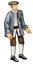
\includegraphics{../data/images/units/Unit0.png}} & Free Colonist & 0 & 3 & 0 & 1\\
%% \raisebox{-10mm}{
\includegraphics{../data/images/units/Unit27.png}} & Indentured Servant & -1 & 3 & 0 & 1\\
%% \raisebox{-10mm}{
\includegraphics{../data/images/units/Unit28.png}} & Petty Criminal & -2 & 3 & 0 & 1\\
%% \raisebox{-10mm}{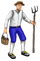
\includegraphics{../data/images/units/Unit1.png}} & Master Farmer & 1 & 3 & 0 & 1\\
%% \raisebox{-10mm}{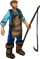
\includegraphics{../data/images/units/Unit2.png}} & Expert Fisherman & 1 & 3 & 0 & 1\\
%% \end{longtable}

\hypertarget{Skills and Education}{\subsection{Skills and Education}}

In FreeCol, your colonists come from all walks of life. Some are
unskilled {\textbf{Petty Criminals}}, who are deported to the
colonies. Others are {\textbf{Indentured Servants}}, or {\textbf{Free
Colonists}} with moderate skills. Still others are masters of their
craft, experts at their trade or profession, who were educated at the
Royal College in Europe. If you have enough gold, you can recruit
units directly from the Royal College.

Not all skills, however, can be learned in Europe. The cultivation of
\hyperlink{Sugar}{Sugar}, \hyperlink{Cotton}{Cotton} and
\hyperlink{Tobacco}{Tobacco}, and the skill of
\hyperlink{Fur}{trapping} are apparently unknown in Europe. Thus,
{\textbf{Master Sugar Planters}}, {\textbf{Master Cotton Planters}},
{\textbf{Master Tobacco Planters}}, as well as the {\textbf{Master Fur
Trappers}}, can not be recruited in Europe.

At the beginning of the game, these skills can only be learned at
Indian Settlements. As soon as you construct a
\hyperlink{Schoolhouse}{Schoolhouse}, however, you can order your
master craftsmen to teach other free colonists their skills. Petty
Criminals and Indentured Servants can not be directly upgraded to
master craftsmen.  However, a Petty Criminal may become an Indentured
Servant, and an Indentured Servant may become a Free Colonist through
education. Petty Criminals may also become Indentured Servants, and
Indentured Servants may also become Free Colonists by winning a battle. 

Indian units are more productive than free colonists when working
outside of the colony, and less productive when working inside a
building. Indian units can not become free colonists through
education, but all Indian units become free colonists as soon as
\hyperlink{Bartolome de las Casas}{Bartolome de las Casas} joins the
\hyperlink{Continental Congress}{Continental Congress}.

\textbf{Scouts} can explore the New World and enter Indian Settlements
in order to speak with the tribal chiefs. A scout entering an Indian
Settlement may become a \textbf{Seasoned Scout} through experience. A
colonist investigating a \hyperlink{Lost City Rumour}{Lost City
Rumour} may also be upgraded to a Seasoned Scout, unless that unit
already has another skill.


\hypertarget{Continental Congress}{\section{Continental Congress}}

As the player generates \hyperlink{Liberty Bells}{Liberty Bells},
{\textbf{Founding Fathers}} are elected to the {\textbf{Continental
Congress}}. The Founding Fathers are historical figures who played a
more or less important part in the conquest of the New World. Each
Founding Father grants the player a new bonus or ability, or causes a
certain event to occur, much like the ``Wonders of the World'' in the
Civilization series. At the beginning of the game, you will need only
a few Liberty Bells to elect a Founding Father to the Continental
Congress, but as the game progresses this number may increase to many
hundred Bells.

\hypertarget{Adam Smith}{\textbf{Adam Smith}} (1723--1790), better
known as the Father of Modern Economics, penned several texts
pertaining to Economic theory, including, ``The Wealth of Nations''
his most famous text. As soon as Adam Smith joins the Continental
Congress, the player is allowed to build factories, which produce 1.5
units of manufactured goods for each unit of raw material consumed.

\hypertarget{Jacob Fugger II}{\textbf{Jacob Fugger II}} (1459--1525)
was an extremely wealthy German merchant and banker who amassed a
fortune with family partnerships and stock holdings in the mining
industries. As soon as Jacob Fugger joins the Continental Congress,
all \hyperlink{boycotts}{boycotts} currently in effect are dropped.

\hypertarget{Peter Minuit}{\textbf{Peter Minuit}} (1580--1638) bought
what later became known as Manhattan Island from Native Americans for
about 60 Dutch guilders. He later colonized the Delware Bay area
as well. As soon as Peter Minuit is elected to the Continental
Congress, the Indians no longer demand payment for their land.

\hypertarget{Peter Stuyvesant}{\textbf{Peter Stuyvesant}} (1592--1672)
was appointed Governor General of the New Netherlands, which, after a
British invasion he could not stop, became New York. With the election
of Peter Stuyvesant, the construction of \hyperlink{Custom
House}{custom houses} becomes possible.

\hypertarget{Jan de Witt}{\textbf{Jan de Witt}} (1625--1672) was a
great Dutch statesmen.  He represented the merchants and a encouraged
industry and commerce. He also negotiated several important treaties
for the Dutch to end wars with England. As soon as Jan de Witt is a
member of the Continental Congress, trade with foreign colonies
becomes possible.

\hypertarget{Ferdinand Magellan}{\textbf{Ferdinand Magellan}}
(1480--1521) was one of the greatest explorers to navigate the
globe. Magellan was first to circumnavigate the globe and cross the
Pacific Ocean. Magellan's election to the Continental Congress
increases the movement of all naval vessels by one, and the time
to sail between Europe and the New World is reduced.

\hypertarget{Fransisco de Coronado}{\textbf{Fransisco de Coronado}}
(1510--1554) was the first European explorer to see the Grand
Canyon. Though he never found the golden cities he searched for, his
mapping of the area now called the Southwestern US was important to
further exploration. As soon as Fransisco de Coronado joins the
Continental Congress, all existing colonies become visible on the map.

\hypertarget{Hernando de Soto}{\textbf{Hernando de Soto}} (1496--1542)
was the first European to explore Florida and the southeastern US.  He
also held a prominent role in conquests of Central America. If
Hernando de Soto is a member of the Continental Congress, the
exploration of \hyperlink{Lost City Rumours}{Lost City Rumours} always
yields a positive result, and all units have an extended sight radius.

\hypertarget{Henry Hudson}{\textbf{Henry Hudson}} (1565--1611) was an
English navigator who explored and mapped a large area of the
northeastern North American continent.  Many waterways in that region
are named in his honour. His original goal was to find the famed
Northwest Passage. The election of Henry Hudson to the Continental
Congress doubles the output of all \hyperlink{Fur Trapper}{Fur
Trappers}.

\hypertarget{Robert La Salle}{\textbf{Robert La Salle}} (1643--1687)
was the first European to travel the length of the Mississippi river,
while on a mission to set up numerous trading posts along its banks.
He later claimed the whole basin as Louisiana in honor of the French
King. Later, he explored several of the Great Lakes. If Robert La
Salle is a member of the Continental Congress, all colonies gain a
stockade as soon as their population reaches three colonists.

\hypertarget{Hernan Cortes}{\textbf{Hernan Cortes}} (1485--1547) was a
famed Spanish conquistador who overthrew the Aztec Empire and claimed
Mexico for Spain. As soon as Hernan Cortes joins the Continental
Congress, conquered native settlements always yield treasure (and in
greater abundance) and the King's \hyperlink{Galleon}{galleons}
transport it free of charge.

\hypertarget{George Washington}{\textbf{George Washington}}
(1732--1799) was the general who lead the colonial army to victory
over the British to gain independence for the colonies. This victory
and his leadership led to his being named the new nation's first
President. If George Washington is a member of the Continental
Congress, any soldier or dragoon who wins a combat is automatically
upgraded to the next possible level.

\hypertarget{Paul Revere}{\textbf{Paul Revere}} (1734--1818) was the
famed rider of colonial America who mounted his horse and rode through
the countryside alerting colonists that British soldiers were
coming. He was captured during the ride and later released when his
captors believed they were in grave danger and their prisoner might
slow them down. With Paul Revere a member of the Continental Congress,
a colonist automatically takes up any stockpiled muskets and defends
an otherwise undefended colony if it is attacked.

\hypertarget{Francis Drake}{\textbf{Francis Drake}} (1542--1596) was a
great English sea captain, the first Englishman to circumnavigate the
globe and a hero in the fights against the Spanish Armada. The
presence of Francis Drake in the Continental Congress increases the
combat strength of all Privateers by 50\%.

\hypertarget{John Paul Jones}{\textbf{John Paul Jones}} (1741--1792)
was hailed as a great sea captain in America, and uttered the famous
words "Sir, I have not yet begun to fight" while fighting the British
at sea. He later watched his ship sink to the bottom of the ocean from
the deck of a British vessel. As soon as John Paul Jones is elected to
the Continental Congress, a \hyperlink{Frigate}{Frigate} is added to
your colonial navy for free.

\hypertarget{Thomas Jefferson}{\textbf{Thomas Jefferson}}
(1743--1826), a powerful voice of patriotism, was credited with
writing the Declaration of Independence. He later became the 3rd
President of the US. The election of Thomas Jefferson to the
Continental Congress increases Liberty Bell production in colonies by
50\%.

\hypertarget{Pocahontas}{\textbf{Pocahontas}} (1595--1617) was a
peacemaker between early Jamestown settlers and the Native
Americans. She is credited with sending food and other supplies to
starving colonists there during harsh times.  She later converted to
Christianity and married an Englishman.  When Pocahontas joins the
Continental Congress, all tension levels between you and natives are
removed and Indian alarm is generated half as fast.

\hypertarget{Thomas Paine}{\textbf{Thomas Paine}} (1737--1809)
inspired colonists with his pen at the urging of Benjamin Franklin. He
published a pamphlet, "Common Sense", guiding the thoughts of patriots
all over the colonies. The election of Thomas Pain to the Continental
Congress increases Liberty Bell production in all your colonies by the
value of the current \hyperlink{Taxes}{tax rate}.

\hypertarget{Simon Bolivar}{\textbf{Simon Bolivar}} (1783--1830) is
remembered as a great leader in the struggle for South American
independence from Spain. Bolivar freed what is now Venezuela and later
became its first President. When Simon Bolivar joins the Continental
Congress, the Sons of Liberty membership in all existing colonies is
increased by 20\%.

\hypertarget{Benjamin Franklin}{\textbf{Benjamin Franklin}}
(1706--1790), a heavy contributor to the Declaration of Independence,
was one of the voices of the Revolution. He traveled extensively
between Europe and the colonies, and gained the support of the French
in the war. As soon as Benjamin Franklin is elected to the Continental
Congress, the King's foreign wars no longer have effect on
relationships in the New World, and Europeans in the New World always
offer peace in negotiations.

\hypertarget{William Brewster}{\textbf{William Brewster}} (1567--1644)
was the Puritan leader of the Plymouth colony in New England. As soon
as William Brewster joins the Continental Congress, criminals or
indentured servants no longer appear on the docks and you can select
which immigrant in the recruitment pool to move to the docks.

\hypertarget{William Penn}{\textbf{William Penn}} (1644--1718), a
close friend of the Duke of York, was granted the land that is mostly
Pennsylvania, Delaware, and New Jersey. He governed the Quaker colony
for several years to provide a haven to fellow Quakers. The election
of William Penn increases cross production in all colonies by 50\%.

\hypertarget{Father Jean de Brebeuf}{\textbf{Father Jean de Brebeuf}}
(1593--1649) founded Quebec City in Canada, befriended the Huron
Indians and converted many to Christianity. He died at the hands of
the Iroquois who had finally defeated their enemy, the Hurons. With
Jean de Brebeuf a member of the Continental Congress, all missionaries
function as experts.

\hypertarget{Juan de Sepulveda}{\textbf{Juan de Sepulveda}}
(1781--1872) was a Spanish missionary who traveled throughout the
Indies converting the Natives to Catholicism and speaking out against
their harsh treatment by Spain. The election of Juan de Sepulveda to
the Continental Congress increases the chance that a subjugated
Indian settlement will ``convert'' and join a colony.

\hypertarget{Bartolme de las Casas}{\textbf{Bartolme de las Casas}}
(1474--1566) was a Catholic Priest who traveled the Indies converting
Indians and chastising Spain for their treatment of the Natives. When
Bartolme de las Casas joins the Continental Congress, all existing
Indian converts become free colonists.




\hypertarget{Copyright Notice}{\section{Copyright Notice}}
Copyright � 2006
\href{http://freecol.sourceforge.net/index.php?section=8}{The FreeCol
Team}.

This manual is free software; you may redistribute it and/or modify it
under the terms of the GNU General Public License as published by the
Free Software Foundation; either version 2, or (at your option) any
later version.

This is distributed in the hope that it will be useful, but without
any warranty; without even the implied warranty of merchantability or
fitness for a particular purpose. See the GNU General Public License
for more details.

A copy of the GNU General Public License is available on the World
Wide Web at \href{http://www.gnu.org/copyleft/gpl.html}{the GNU
General Public Licence}. You can also obtain it by writing to the Free
Software Foundation, Inc., 59 Temple Place - Suite 330, Boston, MA
02111--1307, USA.

\end{document}
